% Kozierok, ch. 17
\chapter{Classful (conventional) addressing}
\label{chap:kozierok-ch17}

The original addressing method for IP addresses divided the IP address
space into five chunks of different sizes called {\emph{classes}}, and
assigned blocks of addresses to organizations from these classes based
on the size and requirements of the organization. In this classful
addressing scheme, each class is reserved for a particular purpose, with
the main address classes differentiated based on how many octets are
used for the network identifier (network ID) and how many are used for
the host identifier (host ID).

In this chapter, I describe classful IP addressing. I begin with an
overview of the concept and general description of the different
classes. I discuss the network and host IDs and address ranges
associated with the different classes. I discuss the capacities of each
of the commonly used classes, meaning how many networks belong to each
and how many hosts each network can contain. I discuss the special
meanings assigned to certain IP address patterns and the special ranges
reserved for private IP addressing, loopback functions, and
multicasting. I conclude with a discussion of the problems with this
type of addressing, which led to it being abandoned in favor of
subnetting, and eventually, classless assignment of the
\protect\hypertarget{ch17.htmlux5cux23idx-CHP-17-0676}{}{}IP address
space.

\subsubsection[Note]{\texorpdfstring{\protect\hypertarget{ch17.htmlux5cux23note-64}{}{}Note}{Note}}

\emph{The classful addressing scheme has been replaced by the classless addressing system described in \vref{chap:kozierok-ch20}.
However, I think it is still important to understand how this original system operates, as it forms the basis for the more sophisticated addressing mechanisms.}



\section{IP classful addressing overview and address classes}

The developers of the Internet Protocol (IP) recognized that organizations come in different sizes and would therefore need varying
numbers of IP addresses on the Internet.
They devised a system to divide the IP address space into {\emph{classes}}, each of which contained a portion of the total addresses and was dedicated to specific uses.
Some classes would be devoted to large networks on the Internet, while others would be reserved for smaller organizations or special purposes.

This original system had no name; it was simply ``the'' IP addressing system.
Today it is called the \emph{classful addressing scheme} to differentiate it from the newer classless scheme.



\subsection{IP address classes}

There are five classes in the classful system, which are assigned the letters~A through~E.
\Cref{tab:ip-address-classes} provides some general information about the classes, their intended uses, and their characteristics.

\begin{table}
   \begin{tabular}{lrrrl}
   \toprule
   class      & fraction & NID & HID & intended use\\
   \midrule
   \textbf{A} & 1/2      & 8   & 24  & Unicast for very large organizations\\
   \textbf{B} & 1/4      & 16  & 16  & Unicast for medium to large organizations\\
   \textbf{C} & 1/8      & 24  & 8   & Unicast for smaller organizations\\
   \textbf{D} & 1/16     & n/a & n/a & IP multicasting\\
   \textbf{E} & 1/16     & n/a & n/a & Reserved for experimental use\\
   \bottomrule
   \end{tabular}
   \caption{IP Address Classes and class Characteristics and Uses}
   \label{tab:ip-address-classes}
\end{table}

Looking at this table (and \cref{fig:ipv4-classes}), you can see that Classes A, B, and C take up most of the total address space (seven-eighths of it).
These are the classes used for {\emph{unicast}} IP addressing and messages sent to a single network interface.
(The blocks also include associated broadcast addresses for these networks.)
This is what I usually consider normal IP addressing.


\begin{figure}
   \centering
   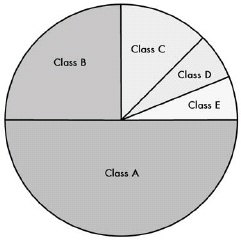
\includegraphics[width=.5\textwidth]{images/ipv4-classes.jpg}
   \caption{Division of IPv4 address space into classes}
   \label{fig:ipv4-classes}
\end{figure}

You can think of Classes A, B, and C as the papa bear, mama bear, and baby bear of traditional IP addressing.
They allow the Internet to provide addressing for a small number of very
large networks, a moderate number of medium-sized organizations, and a
large number of smaller companies. This approximately reflects the
distribution of organization sizes in the real world, though the large
gulf in the maximum number of hosts allowed for each address class leads
to inflexibility, as I will discuss later in the chapter.

As you can see, the classes differ in where they draw the line between
the network ID and the host ID portions of the addresses they contain.
However, in each case, the division is made on octet boundaries. In
classful addressing, the division does not occur within an octet.

Classes D and E are special -- to the point where many people don't even realize they exist.
class D is used for IP multicasting, while class E is reserved for experimental use (by the designers of the Internet).
I discuss IP multicast addressing later in this chapter.


{\textbf{KEY CONCEPT}} The classful IP addressing scheme divides the IP
address space into five classes, A through E, of differing sizes.
Classes A, B, and C are the most important ones, designated for
conventional unicast addresses and taking up seven-eighths of the
address space. class D is reserved for IP multicasting, and class E is
reserved for experimental use.



\subsection{Rationale for classful addressing}

While the drawbacks of the classful system are often discussed today (as
you'll see later in this chapter), it's important to keep in context
what the size of the Internet was when this system was developed. The
Internet was tiny then, and the 32-bit address space seemed enormous by
comparison to even the number of machinesits creators envisioned years
into the future. It's only fair to also remember the following
advantages of the classful system developed over 25 years ago:

\begin{description}
   \item[Simplicity and clarity]
      There are only a few classes to choose from, and it's very simple to understand how the addresses are split up.
      The distinction between classes is clear and obvious.
      The divisions between network ID and host ID in Classes A, B, and C are on octet boundaries, making it easy to tell what the network ID is of any address.

   \item[Reasonable flexibility]
      Three levels of granularity match the sizes of large, medium-sized, and small organizations reasonably well.
      The original system provided enough capacity to handle the anticipated growth rate of the Internet at the time.

   \item[Routing ease]
      As you will see shortly, the class of the address is encoded right into the address to make it easy for routers to know what part of any address is the network ID and what part is the host ID.
      There was no need for adjunct information such as a subnet mask.

   \item[Reserved addresses]
      Certain addresses are reserved for special purposes.
      This includes not just Classes D and E, but also special reserved address ranges for private addressing.
   \end{description}

Of course, it turned out that some of the decisions in the original IP addressing scheme were regrettable -- but that's the benefit of hindsight.
I'm sure we would all like to have back the 268-odd million addresses that were set aside for class E.
While it may seem wasteful now to have reserved a full one-sixteenth of the address space for experimental use, remember that the current size of the Internet was never anticipated even 10 years ago, never mind 25.
Furthermore, it's good practice to reserve some portion of any scarce resource for future use.




\section{IP classful addressing network and host identification and address ranges}

The classful IP addressing scheme divides the total IP address space
into five classes, A through E. One of the benefits of the relatively
simple classful scheme is that information about the classes is encoded
directly into the IP address. This means you can determine in advance
which address ranges belong to each class. It also means the opposite is
possible: You can identify which class is associated with any address by
examining just a few bits of the address. This latter benefit was one of
the main motivators for the initial creation of the classful
system.\protect\hypertarget{ch17s02.htmlux5cux23idx-CHP-17-0685}{}{}


\subsection{Classful addressing class determination algorithm}

When TCP/IP was first created, computer technology was still in its
infancy. Routers needed to be able to quickly make decisions about how
to move IP datagrams around. The IP address space was split into classes
in such a way that, by looking at only the first few bits of any IP
address, the router could easily tell how to choose between the network
and host ID, and thus what to do with the datagram.

The number of bits the router needs to look at may be as few as one or
as many as four, depending on what it finds when it starts looking. The
algorithm used to determine the class corresponds to the system used to
divide the address space, as illustrated in \cref{fig:class-determination}.


\begin{figure}
   \centering
   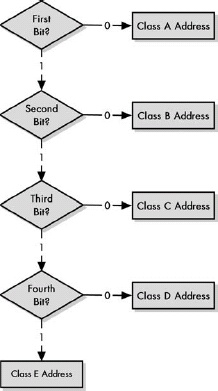
\includegraphics[width=.5\textwidth]{images/class-determination.jpg}
   \caption[Class determination algorithm for classful IP addresses]{Class determination algorithm for classful IP addresses -- The simplicity of the classful IP addressing can be seen in the very uncomplicated algorithm used to determine the class of an address.}
   \label{fig:class-determination}
\end{figure}


Here are the four very basic steps in the algorithm:

\begin{enumerate}
   \item
      If the first bit is a 0, it's a class A address, and you're done.
      (Half the address space has a 0 for the first bit, so this is why class A takes up half the address space.)
      If it's a 1, continue to step 2.
   \item
      If the second bit is a 0, it's a class B address, and you're done.
      (Half of the remaining non-class A addresses, or one quarter of the total.)
      If it's a 1, continue to step 3.
   \item
      If the third bit is a 0, it's a class C address, and you're done.
      (Half again of what's left, or one-eighth of the total.) 
      If it's a 1, continue to step 4.
   \item
      If the fourth bit is a 0, it's a class D address.
      (Half the remainder, or one-sixteenth of the address space.) 
      If it's a 1, it's a class E address.
      (The other half, one-sixteenth.)
\end{enumerate}

And that's pretty much it.



\subsection{Determining address class from the first octet bit pattern}

As humans, of course, we generally work with addresses in dotted decimal
notation and not in binary, but it's pretty easy to see the ranges that
correspond to the classes. For example, consider class B. The first two
bits of the first octet are 10. The remaining bits can be any
combination of ones and zeros. This is normally represented as 10xx xxxx
(shown as two groups of four for readability). Thus, the binary for the
first octet can range from {\textbf{10}}00 0000 to {\textbf{10}}11 1111
(128 to 191 in decimal). So in the classful scheme, any IP address whose
first octet is between 128 and 191 inclusive is a class B address.

\protect\hyperlink{ch17s02.htmlux5cux23ip_address_class_bit_patterns_first-octe}{Table~17-2}
shows the bit patterns for each of the five classes and the way that the first octet
ranges can be calculated. The first column shows the format of the first
octet of the IP address; the {\emph{x}}s can be either a zero or a one.
Next are the lowest and highest value columns for each class in binary
(the fixed few bits are in bold print so you can see that they do not
change while the others do), followed by the corresponding range for the
first octet, in decimal.

\protect\hypertarget{ch17s02.htmlux5cux23ip_address_class_bit_patterns_first-octe}{}{}

Table~17-2.~IP Address class Bit Patterns, First-Octet Ranges, and
Address Ranges

\begin{longtable}[]{@{}lllllll@{}}
\toprule
Class & First octet & Lowest value & Highest value & Range & Octets in Network ID/Host ID & Theoretical IP Address Range\tabularnewline
\midrule
\endhead
class A & \textbf{0}xxx xxxx & {\textbf{0}}000 0001 & {\textbf{0}}111 1110 & 1--127 & 1 / 3 & 1.0.0.0 to 127.255.255.255\\
class B & \textbf{10}xx xxxx & {\textbf{10}}00 0000 & {\textbf{10}}11 1111 & 128--191 & 2 / 2 & 128.0.0.0 to 191.255.255.255\\
class C & \textbf{110}x xxxx & {\textbf{110}}0 0000 & {\textbf{110}}1 1111 & 192--223 & 3 / 1 & 192.0.0.0 to 223.255.255.255\\
class D & \textbf{1110} xxxx & {\textbf{1110}} 0000 & {\textbf{1110}} 1111 & 224--239 & --- & 224.0.0.0 to 239.255.255.255\\
class E & \textbf{1111} xxxx & {\textbf{1111}} 0000 & {\textbf{1111}} 1111 & 240--255 & --- & 240.0.0.0 to 255.255.255.255\\
\bottomrule
\end{longtable}

This table also shows the {\emph{theoretical}} lowest and highest IP
address ranges for each of the classes. This means that they are the
result of taking the full span of binary numbers possible in each class.
In reality, some of the values are not available for normal use. For
example, even though the range 192.0.0.0 to 192.0.0.255 is technically
in class C, it is reserved and not actually used by hosts on the
Internet.

Also, certain IP addresses cannot be used because they have special
meaning. For example, 255.255.255.255 is a reserved broadcast address.

Recall that Classes A, B, and C differ in where the dividing line is
between the network ID and the host ID: 1 for network and 3 for host for
class A, 2 for each for class B, and 3 for network and 1 for host for
class C. Based on this division, in
\protect\hyperlink{ch17s02.htmlux5cux23ip_address_class_bit_patterns_first-octe}{Table~17-2},
I have highlighted the network ID portion of the IP address ranges for
each of Classes A, B, and C. The plain text corresponds to the range of
host IDs for each allowable network ID.
\protect\hyperlink{ch17s02.htmlux5cux23ip_address_class_bit_assignments_and_net}{Figure~17-3}
shows graphically how bits are used in each of the five classes.

\protect\hypertarget{ch17s02.htmlux5cux23ip_address_class_bit_assignments_and_net}{}{}

\protect\hypertarget{ch17s02.htmlux5cux23I_mediaobject3_d1e16900}{}{}
%\includegraphics{httpatomoreillycomsourcenostarchimages287805.png.jpg}

Figure~17-3.~IP address class bit assignments and network/host ID sizes
This illustration shows how the 32 bits of IP address are assigned for
each of the five IP address classes. Classes A, B, and C are the normal
classes used for regular unicast addresses; each has a different
dividing point between the network ID and host ID. Classes D and E are
special and are not divided in this manner.


{\textbf{KEY CONCEPT}} In the classful IP addressing scheme, the class
of an IP address is identified by looking at the first one, two, three,
or four bits of the address. This can be done both by humans working
with these addresses and routers making routing decisions. The use of
these bit patterns means that IP addresses in different classes fall
into particular address ranges that allow an address's class to be
determined by looking at the first byte of its dotted decimal
address.\protect\hypertarget{ch17s02.htmlux5cux23idx-CHP-17-0693}{}{}

For example, consider class C. The lowest IP address is
{\textbf{192.0.0}}.0, and the highest is {\textbf{223.255.255}}.255. The
first three octets are the network ID and can range from
{\textbf{192.0.0}} to {\textbf{223.255.255}}. For each network ID in
that range, the host ID can range from 0 to 255.

\subsubsection[Note]{\texorpdfstring{\protect\hypertarget{ch17s02.htmlux5cux23note-65}{}{}Note}{Note}}

{\emph{It is common to see resources refer to the network ID of a
classful address as including only the significant bits; that is, only
the ones that are not common to all networks of that class. For example,
you may see a class B network ID shown in a diagram as having 14 bits,
with the 10 that starts all such networks shown separately, as if it
were not part of the network ID. Remember that the network ID does
include those bits as well; it is 8 full bits for class A, 16 for Class
B, and 24 for class C. In the case of class D addresses, all 32 bits are
part of the address, but only the lower 28 bits are part of the
multicast group address; see the topic on multicast addressing later in
this chapter for more}}.


\section{IP address class A, B, and C network and host capacities}

So far, I have introduced the concepts of IP address classes and showed
how the classes relate to ranges of IP addresses. Of the five classes, D
and E are dedicated to special purposes, so I will leave those alone for
now. Classes A, B, and C are the ones actually assigned for normal
(unicast) addressing purposes on IP internetworks, and therefore they
are the primary focus of our continued attention.

As you've seen, the classes differ in the number of bits (and octets)
used for the network ID compared to the host ID. The number of different
networks possible in each class is a function of the number of bits
assigned to the network ID, and likewise, the number of hosts possible
in each network depends on the number of bits provided for the host ID.
You must also take into account the fact that one, two, or three of the
bits in the IP address are used to indicate the class itself, so it is
effectively excluded from use in determining the number of networks
(though again, it is still part of the network ID).

Based on this information, you can calculate the number of networks in
each class, and for each class, the number of host IDs per network.
\protect\hyperlink{ch17s03.htmlux5cux23ip_address_class_network_and_host_capaci}{Table~17-3}
shows the calculations.

\protect\hypertarget{ch17s03.htmlux5cux23ip_address_class_network_and_host_capaci}{}{}

Table~17-3.~IP Address Class Network and Host Capacities

\begin{longtable}[]{@{}lllllll@{}}
\toprule
IP Address Class & Total \# of Bits for Network ID/Host ID & First Octet
of IP Address & \# of Network ID Bits Used To Identify Class & Usable \#
of Network ID Bits & Number of Possible Network IDs & \# of Host IDs Per
Network ID\tabularnewline
\midrule
\endhead
{\textbf{class A}} & 8/24 & 0xxx xxxx & 1 & 8-1 = 7 &
2\textsuperscript{7}-2 = 126 & 2\textsuperscript{24}-2 =
16,277,214\tabularnewline
{\textbf{class B}} & 16/16 & 10xx xxxx & 2 & 16-2 = 14 &
2\textsuperscript{14} = 16,384 & 2\textsuperscript{16}-2 =
65,534\tabularnewline
{\textbf{class C}} & 24/8 & 110x xxxx & 3 & 24-3 = 21 &
2\textsuperscript{21} = 2,097,152 & 2\textsuperscript{8}-2 =
254\tabularnewline
\bottomrule
\end{longtable}

Let's walk through one line of this table so you can see how it works
using class B as an example. The basic division is into 16 bits for
network ID and 16 bits for host ID. However, the first 2 bits of all
class B addresses must be 10, so that leaves only 14 bits to uniquely
identify the network ID. This gives us a total of 2\textsuperscript{14}
or 16,384 class B network IDs. For each of these, you have
2\textsuperscript{16} host IDs, less two, for a total of
65,534.\protect\hypertarget{ch17s03.htmlux5cux23idx-CHP-17-0694}{}{}

Why less two? For each network ID, two host IDs cannot be used: the host
ID with all zeros and the ID with all ones. These are addresses with
special meanings, as described in the next section. Also notice that two
is subtracted from the number of network IDs for class A. This is
because two of the class A network IDs (0 and 127) are reserved.

Several other address ranges are set aside in all three of the classes
shown here. They are listed in the ``IP Reserved, Private, and Loopback
Addresses'' section later in this chapter.


{\textbf{KEY CONCEPT}} In the classful IP addressing scheme, a class A
network contains addresses for about 16 million network interfaces; a
class B network contains about 65,000; and a class C network contains
254.

As you can see, there is quite a disparity in the number of hosts
available for each network in each of these classes. What happens if an
organization needs 1,000
\protect\hypertarget{ch17s03.htmlux5cux23idx-CHP-17-0695}{}{}IP
addresses? It must use either four class Cs or one class B (and in so
doing, waste over 90 percent of the possible addresses in the class B
network). Bear in mind that there are only about 16,000 class B network
IDs available worldwide, and you begin to understand one of the big
problems with classful addressing.


\section{IP addresses with special meanings}

Some IP addresses do not refer directly to specific hardware devices; instead, they are used to refer indirectly to one or more devices.
To draw an analogy with language, most IP addresses refer to proper nouns, like ``John'' or ``the red table in the corner.''
However, some are used more the way you use pronouns such as ``this one'' or ``that group over there.''
I call these IP addresses with \emph{special meanings}.

These special addresses are constructed by replacing the normal network ID or host ID (or both) in an IP address with one of two special patterns:

\begin{description}
   \item[All zeros]
      When the network ID or host ID bits are replaced by a set of all zeros, the special meaning is the equivalent of the pronoun \emph{this}, referring to whatever was replaced.
      It can also be interpreted as \emph{the default} or the \emph{current}.
      For example, if you replace the network ID with all zeros but leave the host ID alone, the resulting address means ``the device with the host ID given, on \emph{this network},'' or ``the device with the host ID specified, on \emph{the default network} or \emph{the current network}.''
   \item[All ones]
      When the network ID or host ID bits are replaced by a set of all ones, this has the special meaning of \emph{all}, meaning that the IP address refers to all hosts on the network.
      This is generally used as a broadcast address for sending a message to everyone.
\end{description}

{\textbf{KEY CONCEPT}} When the network ID or host ID of an IP address
is replaced by a pattern of all ones or all zeros, the result is an
address with a special meaning. Examples of such addresses include ``all hosts'' broadcast addresses and addresses that refer to a specific host or a whole network.

There are many special addresses. A small number apply to the entire
TCP/IP network, while others exist for each network or host ID. Since
two special patterns can be applied to the network ID, host ID, or both,
there are six potential combinations, each of which has its own meaning.
Of these, five are used.

\protect\hyperlink{ch17s04.htmlux5cux23ip_address_patterns_with_special_meaning}{Table~17-4}
describes each of these special meanings and includes examples from
class A, B, and C. Note how an IP address in each of the common classes
can be modified to have special meaning forms. (The first row shows the
examples in their normal form, for reference.)

\protect\hypertarget{ch17s04.htmlux5cux23ip_address_patterns_with_special_meaning}{}{}

Table~17-4.~IP Address Patterns with Special Meanings

Network ID

Host ID

class A Example

class B Example

class C Example

Special Meaning and Description

{\textbf{Network ID}}

{\textbf{Host ID}}

77.91.215.5

154.3.99.6

227.82.157.160

{\textbf{Normal Meaning}}: Refers to a specific device.

{\textbf{Network ID}}

{\textbf{All Zeros}}

77.0.0.0

154.3.0.0

227.82.157.0

{\textbf{The Specified Network}}: This notation,
\protect\hypertarget{ch17s04.htmlux5cux23idx-CHP-17-0696}{}{}with a 0 at
the end of the address, refers to an entire network.

{\textbf{All Zeros}}

{\textbf{Host ID}}

0.91.215.5

0.0.99.6

0.0.0.160

{\textbf{Specified Host on This Network}}: This addresses a host on the
current or default network when the network ID is not known or when it
doesn't need to be explicitly stated.

{\textbf{All Zeros}}

{\textbf{All Zeros}}

0.0.0.0

{\textbf{Me}}: Used by a device to refer to itself when it doesn't know
its own IP address. (Alternatively, ``this host,'' or ``the current/default
host.'') The most common use is when a device attempts to determine its
address using a host-configuration protocol like DHCP. May also be used
to indicate that any address of a multihomed host may be used.

{\textbf{Network ID}}

{\textbf{All Ones}}

77.255.255.255

154.3.255.255

227.82.157.255

{\textbf{All Hosts on the Specified Network}}: Used for broadcasting to
all hosts on the local network.

{\textbf{All Ones}}

{\textbf{All Ones}}

255.255.255.255

{\textbf{All Hosts on the Network}}: Specifies a global broadcast to all
hosts on the directly connected network. Note that there is no address
that would imply sending to all hosts everywhere on the global Internet,
since this would be very inefficient and costly.

\subsubsection[Note]{\texorpdfstring{\protect\hypertarget{ch17s04.htmlux5cux23note-66}{}{}Note}{Note}}

{\emph{The missing combination from
\protect\hyperlink{ch17s04.htmlux5cux23ip_address_patterns_with_special_meaning}{Table~17-4}
is that of the network ID being all ones and the host ID normal.
Semantically, this would refer to ``all hosts of a specific ID on all
networks,'' which doesn't really mean anything useful in practice, so
it's not used. Note also that, in theory, a special address where the
network ID is all zeros and the host ID is all ones would have the same
meaning as the all-ones limited broadcast address. The latter is used
instead, however, because it is more general, not requiring knowledge of
where the division is between the network ID and the host ID}}.

Since the all-zeros and all-ones patterns are reserved for these special
meanings, they cannot be used for regular
\protect\hypertarget{ch17s04.htmlux5cux23idx-CHP-17-0697}{}{}IP
addresses. This is why, when you looked at the number of hosts per
network in each of the classes, you had to subtract two from the
theoretical maximum: one for the all-zeros case and one for the all-ones
case.\protect\hypertarget{ch17s04.htmlux5cux23idx-CHP-17-0698}{}{}

Similarly, the network ID cannot be all zeros either. However, this
doesn't require specific exclusion because the entire block of addresses
with 0 in the first octet (0.x.x.x) is one of the reserved sets of
\protect\hypertarget{ch17s04.htmlux5cux23idx-CHP-17-0699}{}{}IP
addresses. These reserved addresses, described in the next section,
further restrict the use of certain addresses in the IP address space
for regular uses.



\section{IP reserved, private, and loopback addresses}

In addition to the unusable numbers with special meanings just
discussed, several other sets of IP addresses have special uses, and are
therefore not available for normal address assignment. These generally
fall into three categories: reserved, private, and loopback addresses.

\subsection{Reserved addresses}

Several blocks of addresses were designated as reserved with no specific
indication given as to what they were reserved for. Perhaps they were
set aside for future experimentation or for internal use in managing the
Internet. (In general, it's a good idea to set aside some portion of any
\protect\hypertarget{ch17s05.htmlux5cux23idx-CHP-17-0700}{}{}limited
resource for unanticipated needs.)

A couple of these blocks appear in each of the three main classes (A, B,
and C), at the beginning and end of each class. (All of class D and E
are also reserved, since they aren't used for regular addressing.)



\subsection{Private, unregistered, nonroutable addresses}

You'll recall that in the IP address overview in \vref{chap:kozierok-ch16}, I contrasted private and
public IP addresses. Every IP address on an IP network must be unique.
In the case of a public IP network, addresses are allocated by a central
authority to ensure that there is no overlap. In contrast, on a private
network, you can use whatever addresses you want.

Then why not just pick any random block of class A, B, or C addresses
for your private network and use that? You could, and some people did.
For example, if you weren't connected to the Internet you could use,
say, the class A network 18.x.x.x that is reserved on the Internet to
the
\protect\hypertarget{ch17s05.htmlux5cux23idx-CHP-17-0701}{}{}Massachusetts
Institute of Technology (MIT). Since you aren't connected to MIT, you
would think that wouldn't matter.

However, as the Internet grew, those disconnected private networks
needed to connect to the public Internet after all, and then they had a
conflict. If they used the 18.x.x.x addresses, they would have to
renumber all their devices to avoid getting a big bunch of computer
geeks really angry. (There were, in fact, cases where companies that had
used IP address space belonging to other companies accidentally
connected those machines to the Internet, causing a small amount of
ruckus in the process.)

RFC 1918 (superseding RFC 1597) provided the solution. It defines a set
of unroutable, special address blocks just for private addresses. These
addresses simply don't exist on the public Internet. For this reason,
they are not registered like other public addresses; they are sometimes
called {\emph{unregistered}}. Anyone can use them, but they cannot
connect to the Internet because routers are not programmed to forward
traffic with these address ranges outside of local organizations. RFC
1918 was published to encourage the use of these private blocks in order
to cut down on the number of devices on the public Internet that didn't
really need to be publicly accessible. This was in response to the need
to conserve the public address space.

\subsubsection[Note]{\texorpdfstring{\protect\hypertarget{ch17s05.htmlux5cux23note-67}{}{}Note}{Note}}

{\emph{In order to connect a network using private addressing to the
public Internet, it is necessary to employ additional hardware and
software. A gateway machine can be used as an interface between the
public and private networks. Technologies such as Network Address
Translation (NAT; see \protect\hyperlink{ch28.html}{Chapter~28}) are
often used in conjunction with private IP addresses to allow these hosts
to communicate on the public IP
network}}.\protect\hypertarget{ch17s05.htmlux5cux23idx-CHP-17-0702}{}{}


{\textbf{KEY CONCEPT}} Private address blocks were created to allow
private IP Internets to be created using addresses that were guaranteed
not to conflict with public IP addresses. They are commonly used in
internetworks that aren't connected to the global Internet; devices
using them can also access the global Internet by using NAT.



\subsection{Loopback addresses}

Normally, when a TCP/IP application wants to send information, that
information travels down the protocol layers to IP, where it is
encapsulated in an IP datagram. That datagram then passes down to the
data link layer of the device's physical network for transmission to the
next hop, on the way to the IP
destination.\protect\hypertarget{ch17s05.htmlux5cux23idx-CHP-17-0703}{}{}

However, one special range of addresses, 127.0.0.0 to 127.255.255.255,
is set aside for {\emph{loopback}} functionality. IP datagrams sent by a
host to a 127.x.x.x loopback address are not passed down to the data
link layer for transmission; instead, they loop back to the source
device at the IP level. In essence, this short-circuits the normal
protocol stack; data is sent by a device's layer~3 IP implementation and
then immediately received by it.

This loopback range is used for testing the TCP/IP protocol
implementation on a host. Since the lower layers are short-circuited,
sending to a loopback address allows you to isolate and test the higher
layers (IP and above) without interference from the lower layers.
\protect\hypertarget{ch17s05.htmlux5cux23idx-CHP-17-0704}{}{}127.0.0.1
is the address most commonly used for testing purposes.


{\textbf{KEY CONCEPT}} Portions of the IP address space are set aside
for reserved, private, and loopback addresses.




\subsection{Reserved, private, and loopback addressing blocks}

\protect\hyperlink{ch17s05.htmlux5cux23reserved_private_and_loopback_ip_address}{Table~17-5}
shows all of the special blocks set aside from the normal
\protect\hypertarget{ch17s05.htmlux5cux23idx-CHP-17-0705}{}{}IP address
space in numerical order, with a brief explanation of how each is used.
It lists both the classful and the classless notation representing each of these blocks because the Internet now uses classless addressing, and because some of the private blocks don't correspond to single class A, B, or C networks.

Note especially the private address block from 192.168.0.0 to 192.168.255.255.
This is the size of a class B network, but it isn't class B in the classful scheme, because the first octet of 192 puts it in the class C part of the address space.
It is actually 256 contiguous class C networks.

You may also notice the special class B (/16) block 169.254.x.x.
This is reserved for {\emph{Automatic Private IP Addressing (APIPA)}}, discussed in
\protect\hyperlink{ch64.html}{Chapter~64}.
Systems that are configured to use this feature will automatically assign systems addresses from this block to enable them to communicate even if no server can be found for proper IP address assignment using the Dynamic Host Control Protocol (DHCP).

\protect\hypertarget{ch17s05.htmlux5cux23reserved_private_and_loopback_ip_address}{}{}

Table~17-5.~Reserved, Private, and Loopback IP Addresses

\begin{longtable}[]{@{}lllll@{}}
\toprule
Range Start Address & Range End Address & Classful Address Equivalent &
Classless Address Equivalent & Description\tabularnewline
\midrule
\endhead
{\textbf{0.0.0.0}} & {\textbf{0.255.255.255}} & class A network 0.x.x.x
& 0/8 & Reserved\tabularnewline
{\textbf{10.0.0.0}} & {\textbf{10.255.255.255}} & class A network
10.x.x.x & 10/8 & class A private address block\tabularnewline
{\textbf{127.0.0.0}} & {\textbf{127.255.255.255}} & class A network
127.x.x.x & 127/8 & Loopback address block\tabularnewline
{\textbf{128.0.0.0}} & {\textbf{128.0.255.255}} & class B network
128.0.x.x & 128.0/16 & Reserved\tabularnewline
{\textbf{169.254.0.0}} & {\textbf{169.254.255.255}} & class B network
169.254.x.x & 169.254/16 & class B private address block reserved for
automatic private address allocation (see
\protect\hyperlink{ch64.html}{Chapter~64} for details)\tabularnewline
{\textbf{172.16.0.0}} & {\textbf{172.31.255.255}} & 16 contiguous Class
B networks from 172.16.x.x through 172.31.x.x & 172.16/12 & class B
private address blocks\tabularnewline
{\textbf{191.255.0.0}} & {\textbf{191.255.255.255}} & class B network
191.255.x.x & 191.255/16 & Reserved\tabularnewline
{\textbf{192.0.0.0}} & {\textbf{192.0.0.255}} & class C network
192.0.0.x & 192.0.0/24 & Reserved\tabularnewline
{\textbf{192.168.0.0}} & {\textbf{192.168.255.255}} & 256 contiguous
class C networks from 192.168.0.x through 192.168.255.x & 192.168/16 &
class C private address blocks\tabularnewline
{\textbf{223.255.255.0}} & {\textbf{223.255.255.255}} & class C network
223.255.255.x & 223.255.255/24 & Reserved\tabularnewline
\bottomrule
\end{longtable}


\section{IP multicast addressing}

The vast majority of traffic on IP internetworks is {\emph{unicast}},
which is one source device sending to one destination device. IP also
supports { \emph{multicasting}}, which is a source device sending to a
group of devices. Multicasting is not used a great deal on the
present-day Internet, mainly due to a lack of widespread hardware
support, though it is useful in certain circumstances, especially as a
more efficient alternative to
broadcasting.\protect\hypertarget{ch17s06.htmlux5cux23idx-CHP-17-0707}{}{}

The classful IP addressing scheme sets aside one-sixteenth of the
address space for
\protect\hypertarget{ch17s06.htmlux5cux23idx-CHP-17-0708}{}{}multicast
addresses as class D. Multicast addresses are identified by the pattern
1110 in the first four bits, which corresponds to a first octet of 224
to 239. Thus, the full range of multicast addresses is from 224.0.0.0 to
239.255.255.255.

Since multicast addresses represent a group of IP devices (sometimes
called a {\emph{host group}}), they can be used only as the destination
of a datagram, never the source.



\subsection{Multicast address types and ranges}

The other 28 bits in the IP address define the {\emph{multicast group
address}}. The size of the class D multicast address space is therefore
2\textsuperscript{28}, or 268,435,456 multicast
\protect\hypertarget{ch17s06.htmlux5cux23idx-CHP-17-0709}{}{}groups. No
substructure defines the use of these 28 bits, and there is no specific
concept of a network ID and host ID as in class A, B, and C. However,
certain portions of the address space are set aside for specific uses.
\protect\hyperlink{ch17s06.htmlux5cux23ip_multicast_address_ranges_and_uses}{Table~17-6}
and
\protect\hyperlink{ch17s06.htmlux5cux23ip_multicast_address_ranges_and_uses_all}{Figure~17-4}
show the general allocation of the class D address
space.\protect\hypertarget{ch17s06.htmlux5cux23idx-CHP-17-0710}{}{}\protect\hypertarget{ch17s06.htmlux5cux23idx-CHP-17-0711}{}{}

\protect\hypertarget{ch17s06.htmlux5cux23ip_multicast_address_ranges_and_uses}{}{}

Table~17-6.~IP Multicast Address Ranges and Uses

\begin{longtable}[]{@{}lll@{}}
\toprule
Range Start Address & Range End Address & Description\tabularnewline
\midrule
\endhead
{\textbf{224.0.0.0}} & {\textbf{224.0.0.255}} & Reserved for special
well-known multicast addresses\tabularnewline
{\textbf{224.0.1.0}} & {\textbf{238.255.255.255}} & Globally scoped
(Internetwide) multicast addresses.\tabularnewline
{\textbf{239.0.0.0}} & {\textbf{239.255.255.255}} & Administratively
scoped (local) multicast addresses\tabularnewline
\bottomrule
\end{longtable}

\subsubsection[Note]{\texorpdfstring{\protect\hypertarget{ch17s06.htmlux5cux23note-68}{}{}Note}{Note}}

{\emph{As with the other IP address classes, the entire 32 bits of the
address is always used. It is only the least significant 28 bits that
are interesting, because the upper four bits never change}}.

\protect\hypertarget{ch17s06.htmlux5cux23ip_multicast_address_ranges_and_uses_all}{}{}

\protect\hypertarget{ch17s06.htmlux5cux23I_mediaobject3_d1e17790}{}{}
%\includegraphics{httpatomoreillycomsourcenostarchimages287807.png.jpg}

Figure~17-4.~IP Multicast address ranges and uses All multicast
addresses begin with 1110. The well-known group has zeros for the first
20 bits of the multicast group address, with 8 bits available to define
255 special multicast addresses. Multicast addresses starting with 1110
1111 are locally scoped; all other addresses are globally scoped (this
includes addresses starting with 1110 0000 other than the 255 well-known
addresses).


{\textbf{RELATED INFORMATION}} {\emph{The concept of multicast address
scope was more completely defined in IPv6, and I discuss it in more
detail in the in the discussion of IPv6 multicast addresses in
\protect\hyperlink{ch25.html}{Chapter~25}}}.

The bulk of the address space is in the middle multicast range. These
are normal multicast addresses, like the class A, B, and C unicast
addresses, and they can be assigned to various groups.

The last address range is for {\emph{administratively scoped}} multicast
groups. This is a fancy term for multicast groups used within a private
organization. This block, representing one-sixteenth of the total
multicast address space, is comparable to the private addresses you saw
earlier in this chapter. It is further subdivided into site-local
multicast addresses, organization-local addresses, and so
forth.

\subsection{Well-known multicast addresses}

The first block of 256 addresses is used to define special, well-known multicast address blocks \cref{tab:link-local-multicast} has a selective listing).
These do not represent arbitrary groups of devices and cannot be assigned in that manner.
Instead, they have a
special meaning that allows a source to send a message to a predefined
group.


\begin{table}
   \centering
   \begin{tabular}{rl}
   \emph{multicast address} & description\\[.75ex]
   \textit{224.0.0.0}       & Reserved; not used\\
   \textit{224.0.0.1}       & All devices on the subnet\\
   \textit{224.0.0.2}       & All routers on the subnet\\
   \textit{224.0.0.3}       & Reserved\\
   \textit{224.0.0.4}       & All routers using DVMRP\\
   \textit{224.0.0.5}       & All routers using OSPF\\
   \textit{224.0.0.6}       & Designated routers using OSPF\\
   \textit{224.0.0.9}       & Designated routers using RIP-2\\
   \textit{224.0.0.11}      & Mobile agents (for Mobile IP)\\
   \textit{224.0.0.12}      & DHCP server/relay agent\\
   \end{tabular}
   \caption{IP multicast addresses for the local subnet}
   \label{tab:link-local-multicast}
\end{table}

Delivery of IP multicast traffic is more complex than unicast traffic due to the existence of multiple recipients.
Instead of the normal resolution method through the Address Resolution Protocol (ARP) used for unicast datagrams, the IP multicast group and a hardware multicast group are mapped.




\section{Problems with classful IP addressing}

The classful addressing system was the first major attempt to define a
method for universal addressing of a large IP internetwork. There was a
reasonable rationale for the system, as I mentioned in the overview of
the classful scheme, and given that it was developed decades ago for a
network that was limited in size, it did the job remarkably well for a
long time.

No one ever expected the Internet to mushroom to anything close to its
current size. As the Internet grew, the classful IP addressing mechanism
showed some problems.

The three main problems with classful addressing are as follows:
\begin{description}
   \item[Lack of internal address flexibility]
      Big organizations are assigned large, monolithic blocks of addresses that aren't a good match for the structure of their underlying internal networks.

   \item[Inefficient use of address space]
      The existence of only three block sizes (Classes A, B, and C) leads to a waste of limited IP address space.

   \item[Proliferation of router table entries]
      As the Internet grows, more and more entries are required for routers to route IP datagrams.
      This causes performance problems for routers.
      Attempting to reduce inefficient address space allocation leads to even more router table entries.
\end{description}

The first issue results primarily from the fact that in the classful
system, big companies are assigned a rather large (class B) or truly
enormous (class A) block of addresses. They are considered by the
Internet routers to be a single network, with one network ID. Now
imagine that you are running a medium-to-large-sized company with 5,000
computers, and you are assigned a class B address for your network. Do
you really have 5,000 computers all hooked into a single network? I sure
as heck hope you don't! Yet you would be forced to try to fit all of
these into a single IP network in the original classful method. There
was no way to create an internal hierarchy of addresses.

The second and third issues both stem from the fact that the
\protect\hypertarget{ch17s07.htmlux5cux23idx-CHP-17-0716}{}{}granularity
in the classful system is simply too low to be practical in a large
internetwork; there are simply too few choices in the sizes of available
networks. Three sizes seem fine in principle, but the gaps between the
sizes are enormous, and the sizes don't match up well with the
distribution of organizations in the real world. Consider the difference
in size between class C and class B networks -- a jump from 254 hosts all
the way up to over 65,000! There are many, many companies that need more
than 254 IP address but a lot fewer than 65,000. And what about class A?
How many companies need 16 {\emph{million}} IP addresses, even the truly
large ones? Probably none, if you think about it, yet that's half the IP
address space right there.

What class of network should the company with 5,000 computers use? As
\protect\hyperlink{ch17s07.htmlux5cux23the_main_problem_with_classful_addressin}{Figure~17-5}
shows, the classful scheme offers no good match for this company's
needs. If it were assigned a class B, over 90 percent of the IP
addresses would be wasted.

The alternative to wasting all these IP addresses would be to give this
fictitious company a bunch of class C addresses instead of one class B;
but they would need 20 of them. While this would use the address space
more efficiently, it leads to the third issue: Every router on the
Internet then has to replace the single class B router table entry with
20 class C router entries. Multiply this by a few thousand medium-sized
companies, and you can see that this method would add dramatically to
the size of router tables. The larger these tables, the more time it
takes for routers to make routing decisions.

\protect\hypertarget{ch17s07.htmlux5cux23the_main_problem_with_classful_addressin}{}{}

\protect\hypertarget{ch17s07.htmlux5cux23I_mediaobject3_d1e17980}{}{}
%\includegraphics{httpatomoreillycomsourcenostarchimages287809.png.jpg}

Figure~17-5.~The main problem with classful addressing In this scale
diagram, each square represents 50 available addresses. Since a class C
address has only 254 addresses, and a class B contains 65,534 addresses,
an organization with 5,000 hosts is caught in the middle. It can only
choose to either waste 90 percent of a class B address or use 20
different class C networks.

The problems with classful addressing have been solved by three
enhancements, as you'll see in later chapters. The first, which
primarily addresses the first issue, was the development of subnetting.
The second was the move to classless addressing and routing, which
replaces the classful system with a new method with higher granularity.
This tackles the second and third issues by letting addresses be
assigned based on real organizational needs, without requiring numerous
routing table entries for each organization. The third improvement is
the new IP version 6 (IPv6), which finally does away with the cramped
32-bit IP address space in favor of a gargantuan 128-bit one.

Other support technologies, such as NAT, have helped to extend the life
of IPv4 by allowing multiple devices to share public addresses. This
alone has added years to the life of the IPv4 addressing system.
